%!TEX encoding = ISO-8859-1

%\documentclass[%
%\papersize,
%10pt,%
%a4paper,
%%showtrims%
%]{memoir}

\documentclass[a4paper,twoside]{memoir}


% metadata
\title{Ethnogeographic Recognition Through Facial Feature Classification}
\author{Lee Archer}
\date{2014 - 2015}

% packages:
\XeTeXinputencoding latin1
\usepackage[usenames,dvipsnames]{xcolor}
\usepackage[latin1]{inputenx}
\usepackage[T1]{fontenc}
\usepackage[english]{babel}
\usepackage[square]{natbib}\citeindextrue
\usepackage{graphicx}
\usepackage{color}
\usepackage{tikz,pgf}
\usepackage{amsmath,amssymb,theorem}
\usepackage{url}
\usepackage{listings}
\usepackage{multirow}
\usepackage{booktabs}
\usepackage{xspace}
\usepackage{cancel}
\usepackage[printonlyused,withpage,footnote]{acronym}

\usepackage{rotating}
\usepackage{cite}
\usepackage{array}
\usepackage[htt]{hyphenat}
\usepackage{hyperref}
\usepackage{fontspec}
\usepackage{wrapfig}
\usepackage{caption}
\usepackage{subcaption}
\usepackage{minted}
\usepackage[noabbrev]{cleveref}

\copypagestyle{thesis}{Ruled}
\pagestyle{thesis}
\makeevenfoot{thesis}{}{\thepage}{} %
\makeoddfoot{thesis}{}{\thepage}{}  %


% notes
\usepackage{xargs}                      
\usepackage[colorinlistoftodos,prependcaption,textsize=tiny]{todonotes}
\newcommandx{\unsure}[2][1=]{\todo[linecolor=red,backgroundcolor=red!25,bordercolor=red,#1]{#2}}
\newcommandx{\change}[2][1=]{\todo[linecolor=blue,backgroundcolor=blue!25,bordercolor=blue,#1]{#2}}
\newcommandx{\info}[2][1=]{\todo[linecolor=OliveGreen,backgroundcolor=OliveGreen!25,bordercolor=OliveGreen,#1]{#2}}
\newcommandx{\improvement}[2][1=]{\todo[linecolor=Plum,backgroundcolor=Plum!25,bordercolor=Plum,#1]{#2}}
\newcommandx{\improvements}[2][1=]{\todo[noprepend,linecolor=Plum,backgroundcolor=Plum!25,bordercolor=Plum,#1]{ \begin{minipage}{\textwidth-12pt}#2\end{minipage}  }}
\newcommandx{\thiswillnotshow}[2][1=]{\todo[disable,#1]{#2}}

% minted
\newmintedfile[yamlfile]{yaml}{
    fontfamily=tt,
    fontsize=\scriptsize,
    linenos=true,
    numberblanklines=true,
    numbersep=12pt,
    numbersep=5pt,
    gobble=0,
    frame=leftline,
    framerule=0.4pt,
    framesep=2mm,
    funcnamehighlighting=true,
    tabsize=4,
    obeytabs=false,
    mathescape=false
    samepage=false, %with this setting you can force the list to appear on the same page
    showspaces=false,
    showtabs =false,
    texcl=false,
}

% pdf
\hypersetup{bookmarks, colorlinks, breaklinks, pdftitle={Ethnogeographic 
    Recognition Through Facial Feature Classification},pdfauthor={Lee Archer},
  linkcolor=black,citecolor=black,filecolor=black,urlcolor=black}

% other metadata
\newcommand{\polimi}{University of Bristol\xspace}
\newcommand{\dei}{Department of Computer Science\xspace}
\newcommand{\address}{Woodland Road, Clifton, Bristol BS8 1UB\xspace}
\newcommand{\POLIMI}{\uppercase{\polimi}}
\newcommand{\DEI}{\uppercase{\dei}}

% fonts
\newcommand{\XeTeX}{{\normalsize X\textsubscript{\footnotesize E}T\textsubscript{\footnotesize E}X}\xspace}
\newcommand{\nfont}{Adobe Caslon Pro}
\newcommand{\ttfont}{Envy Code R}
\newcommand{\sffont}{Oregon LDO}
\newcommand{\commodorefont}{Commodore 64 Pixeled}
\defaultfontfeatures{Mapping=tex-text}
\setromanfont[Ligatures={Common}]{\nfont}
\setmonofont[Scale=0.8]{\ttfont}
\setsansfont[Scale=0.9]{\sffont}

%acronyms
%\renewcommand*{\acfsfont}[1]{{\normalsize\upshape #1}}
%\renewcommand*{\acffont}[1]{{\normalsize\itshape #1}}
%\renewcommand{\vec}[1]{\mathbf{#1}}


% hypenations
\hyphenation{a-no-ma-lous a-no-ma-ly lib-a-no-ma-ly web-a-no-ma-ly group-ed fuzz-ing a-mo-unts bre-ach-es well-trai-ned trai-ned data-set data-sets a-gain-st}

% graphics
\usetikzlibrary{patterns,shadows,automata,calc,arrows,shapes,backgrounds,fit,trees}
\definecolor{c64}{rgb}{.063,0,.612}
\definecolor{c64light}{rgb}{.451,.451,1}

% layout:
% w = 297mm
% P =~ sqrt(2)
% s = 297/8 (spine)
% t = 297/8 (top)
% e = 297/4 (fore-edge)
% f = 297/4 (foot)
%\setstocksize{24cm}{17cm}
%\settrimmedsize{24cm}{17cm}{*}
\setlrmarginsandblock{4cm}{3cm}{*}
\setulmarginsandblock{1in}{*}{*}
\setmarginnotes{17pt}{51pt}{\onelineskip}
\setheadfoot{\onelineskip}{2\onelineskip}
\setheaderspaces{*}{2\onelineskip}{*}
\setlength{\trimtop}{0pt}
\setlength{\trimedge}{\stockwidth}
\addtolength{\trimedge}{-\paperwidth}
\checkandfixthelayout


% chapter style:
\makeatletter
\makechapterstyle{thesis}{%
  \renewcommand{\chapternamenum}{}
  \setlength{\beforechapskip}{0pt}
  \setlength{\midchapskip}{0pt}
  \setlength{\afterchapskip}{0pt}
  \renewcommand{\chapnamefont}{\LARGE}
  \renewcommand{\chapnumfont}{\chapnamefont}
  \renewcommand{\chaptitlefont}{\chapnamefont}
  \renewcommand{\printchapternum}{}
  \renewcommand{\afterchapternum}{}
  \renewcommand{\printchaptername}{}
  \renewcommand{\afterchaptertitle}{\chapnumfont\hfill\thechapter\\\vspace*{-.3cm}\hrulefill\vspace*{6cm}\\}
}
\makeatother

% titles:
\renewcommand{\maketitlehooka}{%
  \centering
  
\includegraphics[width=6cm]{figures/bristol-logo}\\[.5cm]
  \POLIMI\\
  \emph{\dei}\\[.2cm]
  \par
  \hrulefill
  \vfill}
\renewcommand{\maketitlehookb}{\vfill}
\renewcommand{\maketitlehookc}{%
  \vfill
  \begin{flushleft}
    Tutor:\\
    \textbf{Prof. Peter Flach}\\[.3cm]
    Supervisor:\\
    \textbf{Dr. Tilo Burghardt}
  \end{flushleft}
  \vfill}
\preauthor{\begin{flushright}Bachelor of Science Thesis of:\\\bfseries}
\postauthor{\end{flushright}}

% divisions:
\maxsecnumdepth{subsubsection}
\maxtocdepth{subsection}

\makeatletter 
\renewcommand{\fnum@figure}{\textsc{\figurename~\thefigure}}
\makeatother

% math
\DeclareMathOperator{\Score}{Score}
\DeclareMathOperator{\stdev}{stdev}
\DeclareMathOperator{\BMU}{BMU}
\newcommand{\mtok}{m^{\left(\text{tok}\right)}}
\newcommand{\minty}{m^{\left(\text{int}\right)}}
\newcommand{\mdoc}{m^{\left(\text{doc}\right)}}
\newcommand{\msess}{m^{\left(\text{sess}\right)}}
\newcommand{\mlen}{m^{\left(\text{len}\right)}}
\newcommand{\mchar}{m^{\left(\text{char}\right)}}
\newcommand{\mstruct}{m^{\left(\text{struct}\right)}}
\newcommand{\kb}{\mathcal{C}}

\newcommand{\qed}{\blacksquare}

\theoremstyle{plain}
\newtheorem{thm}{Theorem}[section]
\newtheorem{prop}[thm]{Proposition}
\newtheorem{proof}{Proof}[section]

\theorembodyfont{\rmfamily}
\newtheorem{definition}{Definition}[section]
\newtheorem{example}{Example}[section]

\newtheorem{rem}{Remark}
\newtheorem{note}{Note}[section]

\makeatletter
\newif\if@borderstar
\def\bordermatrix{\@ifnextchar*{%
    \@borderstartrue\@bordermatrix@i}{\@borderstarfalse\@bordermatrix@i*}%
}
\def\@bordermatrix@i*{\@ifnextchar[{%
    \@bordermatrix@ii}{\@bordermatrix@ii[()]}
}
\def\@bordermatrix@ii[#1]#2{%
  \begingroup
  \m@th\@tempdima8.75\p@\setbox\z@\vbox{%
    \def\cr{\crcr\noalign{\kern 2\p@\global\let\cr\endline }}%
    \ialign {$##$\hfil\kern 2\p@\kern\@tempdima & \thinspace%
      \hfil $##$\hfil && \quad\hfil $##$\hfil\crcr\omit\strut%
      \hfil\crcr\noalign{\kern -\baselineskip}#2\crcr\omit%
      \strut\cr}}%
  \setbox\tw@\vbox{\unvcopy\z@\global\setbox\@ne\lastbox}%
  \setbox\tw@\hbox{\unhbox\@ne\unskip\global\setbox\@ne\lastbox}%
  \setbox\tw@\hbox{%
    $\kern\wd\@ne\kern -\@tempdima\left\@firstoftwo#1%
      \if@borderstar\kern2pt\else\kern -\wd\@ne\fi%
      \global\setbox\@ne\vbox{\box\@ne\if@borderstar\else\kern 2\p@\fi}%
      \vcenter{\if@borderstar\else\kern -\ht\@ne\fi%
        \unvbox\z@\kern-\if@borderstar2\fi\baselineskip}%
      \if@borderstar\kern-2\@tempdima\kern2\p@\else\,\fi\right\@secondoftwo#1 $%
  }\null \;\vbox{\kern\ht\@ne\box\tw@}%
  \endgroup
}
\makeatother

% code:
\lstset{
  basicstyle=\ttfamily\small,
  basewidth=0.55em,
  showstringspaces=false,
  numbers=left,
  numberstyle=\tiny,
  numbersep=2.5pt,
  keywordstyle=\bfseries\ttfamily,
  breaklines=true
}
\lstnewenvironment{pseudoc}{\lstset{frame=lines,language=C,mathescape=true}}{}
\lstnewenvironment{logs}{\lstset{frame=lines,basicstyle=\footnotesize\ttfamily,numbers=none}}{}
\lstnewenvironment{cc}{\lstset{frame=lines,language=C}}{}
\lstnewenvironment{c64}{\lstset{backgroundcolor=\color{c64},basewidth=0.65em,basicstyle=\commodoreface\color{c64light},numbers=none,framerule=10pt,rulecolor=\color{c64light},frame=tb,framexbottommargin=30pt}}{}
\lstnewenvironment{html}{\lstset{frame=lines,language=html,numbers=none}}{}
\lstnewenvironment{pseudo}{\lstset{frame=lines,mathescape=true,morekeywords={learn_string_domain, save_model}}}{}

\lstnewenvironment{pseudoctiny}{\lstset{language=C,mathescape=true,basicstyle=\tiny\sffamily}}{}
\lstnewenvironment{cctiny}{\lstset{language=C,basicstyle=\tiny\sffamily}}{}
\lstnewenvironment{pseudotiny}{\lstset{mathescape=true,basicstyle=\tiny\sffamily}}{}

% definitions:
\newcommand{\SSAADE}{S\textsuperscript{2}A\textsuperscript{2}DE\xspace}
\newcommand{\SyscallAnomaly}{\index{SyscallAnomaly}\textsf{Sys\-call\-A\-no\-ma\-ly}\xspace}
\newcommand{\LibAnomaly}{\index{LibAnomaly}\textsf{Lib\-A\-no\-ma\-ly}\xspace}
\newcommand{\webanomaly}{\index{webanomaly}\textsf{web\-a\-no\-ma\-ly}\xspace}
\newcommand{\masibty}{\index{Masibty}\textsf{Masibty}\xspace}

\makeindex

\begin{document}

\selectlanguage{english}

\begin{titlingpage}
  \maketitle
\end{titlingpage}

\frontmatter

\section*{Declaration}
A dissertation submitted to the University of Bristol in 
accordance with the requirements of the degree of Bachelor of Science in 
the Faculty of Engineering. It has not been submitted for any other 
degree or diploma of any examining body. Except where 
specifically acknowledged, it is all the work of the Author. 

\begin{flushright}
  \textsc{\theauthor}\\
  Bristol\\
  July 2015
\end{flushright}

%%% Local Variables: 
%%% mode: latex
%%% TeX-master: "thesis"
%%% End: 


\cleartoverso

\begin{abstract}
    Abstract placeholder.
\end{abstract}


%%% Local Variables: 
%%% mode: latex
%%% TeX-master: "thesis"
%%% End: 


\cleartoverso

\selectlanguage{english}

\cleartoverso

\tableofcontents*

\mainmatter

\chapterstyle{thesis}


\chapter{Introduction}
\label{introduction}

% Biological aspects
Race has been a significant issue throughout the history of humans 
and a source of many conflicts, however from a biological point of view
there are no distinct, pure races in humans, despite the vast diversity 
in visual traits of people from different parts of the world.
% cite: http://www.physanth.org/about/position-statements/biological-aspects-race/

Nonetheless, we have always been keen to find patterns in nature and 
classify living beings. The number of major racial groups varies from 
one source to the other, but they are still recorded as a part of censuses 
in many countries to identify racial disparities in social and economic aspects.
% cite: http://www.census.gov/topics/population/race/about.html

People living in multicultural countries such as the United States and the 
United Kingdom can often distinguish between people whose origins trace to other
parts of the world if their ancestors have not mixed with other races.

For example, it would be quite trivial for them to correctly identify if some person
originates from Africa, East Asia or Europe. This can be done just by looking and
analysing the person's face as it contains many important cues such as skin colour, 
shape of the nose, distance between the eyes and many others.

There have been many successful attempts at creating computer systems that can perform
this task using images of human faces with striking accuracy. One of the 
most useful papers for this project was \citep{muhammadg} which reviews 
race classifiers using 2, 3 or 4 classes (major races) with accuracies 
ranging from \textbf{X} to \textbf{Y}.

The aim of this project was to go further and predict a much narrower ethnic group 
of a person by analysing images of their face. This is a far more challenging task 
as different ethnic groups within the same race have significantly more common 
facial features and visual similarities than ethnic groups from different races.

Surprisingly, there were not many studies done about this sub-class of the race 
recognition problem.

% discuss the Chinese ethnic groups study





\section{Popular datasets for race recognition}
\label{introduction:datasets}
General discussion of popular race recognition datasets.
\subsection{Example}
\label{introduction:datasets:example}
Dataset called Example.

\section{Choosing a dataset for this experiment}
\label{introduction:ourdataset} 
Our dataset placeholder.

\section{Document Structure}
\label{introduction:structure} 
Structure placeholder.
%This document is structured as
%follows. Chapter~\ref{detection} introduces the \ac{ID}, that is the
%topic of our research. In particular, Chapter~\ref{detection}
%rigorously describes all the basic components that are necessary to
%define the \ac{ID} task and an \acp{IDS}. The reader with knowledge on
%this subject may skip the first part of the chapter and focus on
%Section~\ref{detection:ad} and \ref{detection:correlation} that
%include a comprehensive review of the most relevant and influential
%modern approaches on network-, host-, web-based \ac{ID} techniques,
%along with a separate overview of the alert correlation approaches.

%As described in Section~\ref{introduction:contributions}, the
%description of our contributions is structured into three
%chapters. Chapter~\ref{host} focuses on host-based techniques,
%Chapter~\ref{web} regards web-based anomaly detection, while
%Chapter~\ref{correlation} described two techniques that allow to
%recognize relations between alerts reported by network- and host-based
%systems. Reading Section~\ref{detection:ad:network} is recommended
%before reading Chapter~\ref{correlation}.

%The reader interested in protection techniques for the operating
%system can skim through Section~\ref{detection:ad:host} and then read
%Chapter~\ref{host}. The reader with interests on web-based protection
%techniques can read Section~\ref{detection:ad:web} and then
%Chapter~\ref{web}. Similarly, the reader interested in alert
%correlation systems can skim through
%Section~\ref{detection:ad:network} and \ref{detection:ad:host} and
%then read Chapter~\ref{correlation}.

%%% Local Variables: 
%%% mode: latex
%%% TeX-master: "thesis"
%%% End: 


%\let\stdsection\section
%\renewcommand\section{\newpage\stdsection}

\chapter{Background and literature review}
\label{background}
Background placeholder.

%%% Local Variables: 
%%% mode: latex
%%% TeX-master: "thesis"
%%% End: 

\chapter{Specification and system design}
\label{spec}
\section{Data collection}
The quantity and the quality of training data is crucial to all computer vision 
projects. However, for this task there was no luxury of using an existing 
dataset with the required level of detail in labels that would also be 
affordable.

A decision was made to collect own data for this project from a social network 
that makes it easy to associate user profiles with photos of themselves with 
locations accurate to city-level. Popular social networks such as Facebook 
would be ideal for this, however it is not possible to obtain a list of 
profiles from a hand-picked location due to Facebook API constraints. 
Moreover, it is clearly stated in Facebook's Terms and Conditions that any way 
to circumvent these constraints would still count as a violation.


\subsection{Tinder}
Tinder is a mobile dating application that shows profiles closest to the 
user's GPS location. There have been numerous third-party Tinder utilities on 
the Web that reverse-engineered Tinder's simple and unobfuscated HTTP API that 
makes it possible to create a fully-featured Tinder client yourself.

The API has support for various actions such as liking and messaging users, 
but for the purposes of this project, the only relevant actions to us are 
authentication, setting own location using latitude and longitude coordinates 
and fetching nearby users.

Tinder profiles are created using Facebook Login. When the application is 
opened for the first time by a non-registered user, they will be prompted to 
login using their Facebook account which gives Tinder access to the user's full name, 
age, pictures and other details.

A user profile was created specifically for this project using the original 
Tinder mobile application on an Android phone. 

\subsection{Profile metadata and photo collection}
A web application (\texttt{tinder-gather}) was written to mimic the Tinder app whose only purpose was 
to record profile metadata such as name, location and date birth as well as 
to save user-uploaded pictures. 

This web application provides an API that allows an external tool 
(\ref{spec:data:jobs}) to easily change the location of the user for this 
application so that images are collected from several different 
countries.

The web application must be used with a complementary Chrome extension 
(\texttt{tinder-gather-connect}) that handles Facebook authentication.
Once the extension is installed a button to launch the app will appear in the 
toolbar. As soon as the user signs in the app will be ready to accept data 
collection jobs from the Tinder job manager tool (\ref{spec:data:jobs}).

\subsection{Tinder job manager}
\label{spec:data:jobs}
Images of people need to be collected from a number of different locations 
around the world. Specifying the coordinates of each location using latitude 
and longitude values proved to be cumbersome in the beginning which is why a 
special and user-friendly tool was written to manage data collection from the 
command line.

This tool resides in the \texttt{tinder-gather} project in the \texttt{tools} 
directory. Usage and help will be displayed in the terminal if ran with these 
arguments:
\begin{logs}
./jobs.js tjob post
\end{logs}

This command expects three arguments: location, limit and delay. Location is 
just a city name whose location is hard-coded inside the script and can be 
easily extended. This argument is required. Limit refers to the maximum number 
of profiles to fetch from Tinder at once and delay specifies how frequently 
they will be fetched.

This tool is also used to manage face and landmark detection jobs which will 
be described in detail in Section \ref{spec:fd}. 

\section{Face and landmark detection}
\label{spec:fd}
Before the collected pictures of faces from different parts of the world 
could be used to learn how to determine the location of a person from a single 
picture of their face they must first be heavily filtered as many Tinder users 
upload very low-quality pictures or even pictures of pets and inanimate 
objects.

A face detector is an ideal method of filtering out non-face images as well as
heavily edited or poor quality face pictures. 

Viola-Jones is the most popular choice for face detection due to its 
incredible performance and native implementation in OpenCV, but it falls 
behind some other face detection algorithms such as those used by 
Google Picasa and face.com.

Unfortunately, Google Picasa and face.com use closed-source 
solutions making them unsuitable for use in this project. However, it was 
discovered that there is an open face detection model that comes very close 
to these commercial algorithms and significantly outperforms Viola-Jones at
the face detection task.

The model can also be trained to learn landmark localisation and face angle, 
which provide additional information that enables us to further filter and 
preprocess the images collected from Tinder profiles. This is important 
because being able to estimate the locations of certain landmarks such as eyes 
makes it possible to scale and rotate images so that the landmarks line up.

Another advantage of this particular solution is that it comes with 
pre-trained on the MultiPIE dataset which needs to be purchased. 

\subsection{Face, landmark and pose detection using mixture of trees and HoG}
...

\section{Preprocessing}
\label{spec:preproc}
The problem with using unprocessed Tinder profile pictures is that they are 
taken at a variety of different angles and scales. Before these pictures can 
be used to train a classifier they must first be transformed so that they all 
have the same angle and scale. This was done by using previously detected 
locations of eyes as reference points so that they always appear in the same 
location in the image. 

\begin{equation}
\label{eq:a}
\alpha = \arccos{\frac{v_{i} \cdot v_{ref}}{|v_{i}| |v_{ref}|}}
\end{equation}


 
\section{Feature extraction}


\section{Classification}

%%% Local Variables: 
%%% mode: latex
%%% TeX-master: "thesis"
%%% End: 

\chapter{Implementation}
\label{impl}
\section{Data collection}
The entire data collection suite is written in JavaScript for Node.js and can 
be found in the \texttt{tinder-gather} directory. The Google Chrome extension 
is also written in JavaScript and the name of its project directory is 
\texttt{tinder-gather-connect}.

\texttt{tinder-gather} is a web application which was made possible using the 
Express.js web application framework. It provides a RESTful HTTP API to manage 
data collection jobs as well as a few debugging pages for viewing face 
detection results.

Profiles and user images found using a modified version of the Tinder.js 
library that implements the Tinder API are stored on disk in the 
\texttt{tinder-gather/gather-images} directory. The metadata for both profiles 
and images is stored in a PostgreSQL database using an ORM library called 
Sequelize, which means it can be easily swapped for an alternative SQL 
database.

Figure \ref{fig:impl:erd_basic} shows the ER diagram for the data collection-
specific part of the database as well as entity \texttt{Detection Job} which 
will be covered in Section \ref{impl:fd}.

The names in parentheses correspond to the actual, case-sensitive table names 
in the PostgreSQL database. 
\begin{figure}[t]
  \centering
  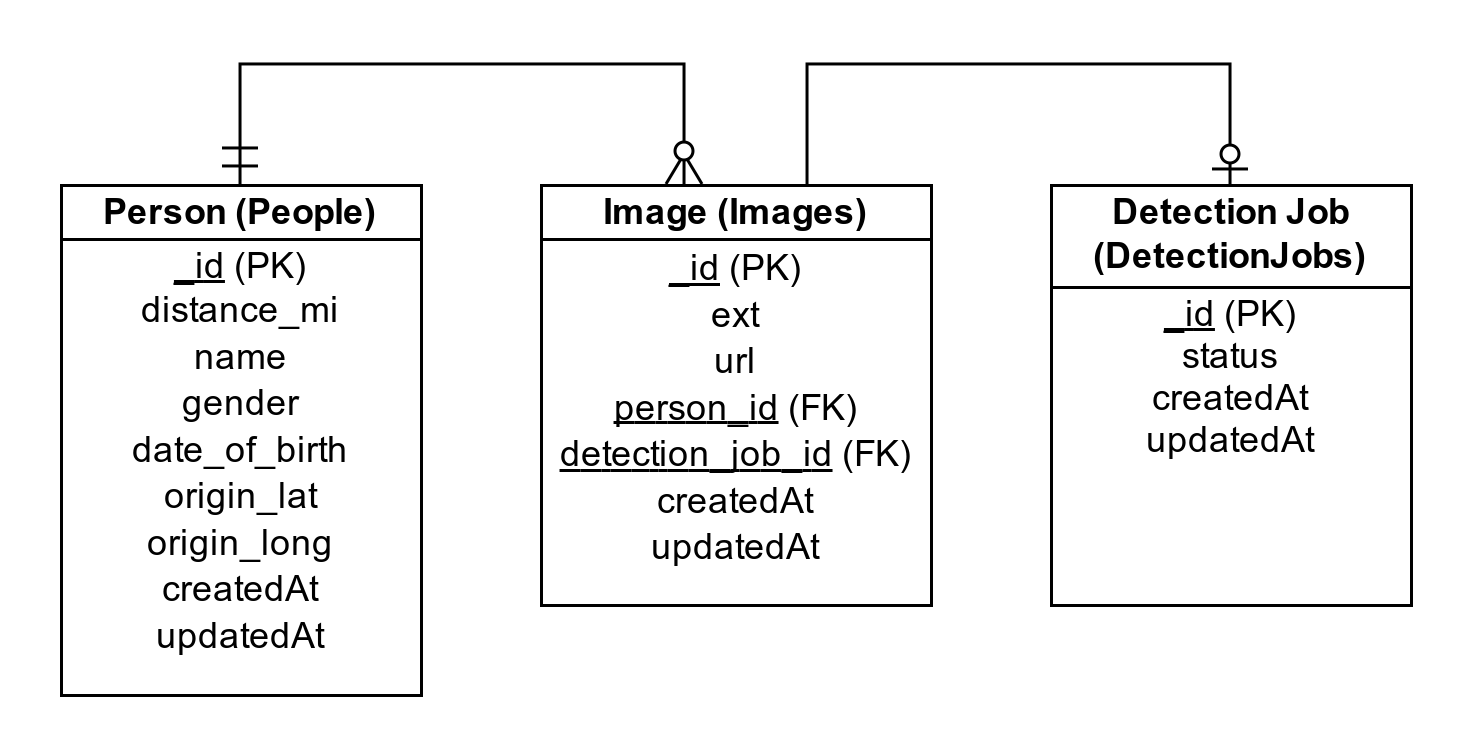
\includegraphics[width=\textwidth]{figures/impl/erd_basic}
  \caption{Entity-relation diagram for tables used by the data collection 
  application \texttt{tinder-gather}. }
  \label{fig:impl:erd_basic}
\end{figure}

\begin{table}[t]
    \begin{center}
        \begin{tabular}{ c  c  c }
            \toprule
            Attribute       & Data type              & Other \\ \toprule
            \multicolumn{3}{c}{Person (People)} \\ \midrule
            \_id           & character(24)            & not null   \\ 
            distance\_mi   & integer                  &            \\ 
            name          & character varying(255)   &            \\ 
            gender        & integer                  &            \\ 
            date\_of\_birth & integer                  &            \\ 
            origin\_lat    & double precision         &            \\ 
            origin\_long   & double precision         &            \\ 

            \midrule
            \multicolumn{3}{c}{Image (Images)} \\ \midrule
            \_id              & character(36)            & not null   \\ 
            ext              & character varying(4)     &            \\ 
            url              & character varying(255)   &            \\ 
            person\_id        & character(24)            &            \\ 
            detection\_job\_id & integer                  &            \\ 

            \midrule
            \multicolumn{3}{c}{Detection Job (DetectionJobs)} \\ \midrule
            \_id      & integer                     & not null, auto-increment \\ 
            status    & enum{started, finished}      &         \\ 

            \midrule
            \multicolumn{3}{c}{Common among all tables} \\ \midrule
            createdAt & timestamp with time zone     & not null  \\ 
            updatedAt & timestamp with time zone     & not null  \\  \bottomrule
        \end{tabular}
    \end{center}
    \caption{Attribute data types of entities introduced in Figure 
    \ref{fig:impl:erd_basic}}
    \label{table:impl:erd_basic_dt}
\end{table}
\subsection{Authentication}
A Google Chrome extension was written in order to obtain an authentication 
token for the Tinder app on Facebook which must be sent with every request to 
the Tinder API. The extension adds a button to the Google Chrome toolbar which 
opens a static web page that sends a request back to the extension to open the 
following URL:
\begin{logs}
https://www.facebook.com/v2.0/dialog/oauth
    ?response_type=token
    &display=popup
    &api_key=464891386855067
    &redirect_uri=fbconnect%3A%2F%2Fsuccess
    &scope=user_about_me%2Cuser_activities%2Cuser_education_history%2Cuser_location%2Cuser_photos%2Cuser_relationship_details%2Cuser_status'
\end{logs}
where \texttt{api\_key} specifies the Tinder application ID on Facebook and 
\texttt{scope} lists the type of information Tinder will gain access to. This 
page asks the user to sign in with their Facebook credentials and, if 
successful, will save a cookie that will be sent along with the next request:

\begin{logs}
POST https://www.facebook.com/v2.0/dialog/oauth/confirm

{
  "app_id: "464891386855067",
  "ttstamp: "2658170904850115701205011500",
  "redirect_uri": "fbconnect://success",
  "return_format": "access_token",
  "from_post": 1,
  "display": "popup",
  "gdp_version": 4,
  "sheet_name": "initial",
  "__CONFIRM__": 1
}
\end{logs}
The response to this will contain an access token that will be used to 
interact with the Tinder API. It can be extracted using 
\begin{logs}
    access_token=([\w_]+)&
\end{logs} 
as a regular expression. It will be referred to as \texttt{<fb\_token>} from 
this point on.

Before we can use it to authenticate with Tinder the Facebook user ID must 
also be obtained by accessing 
\texttt{https://graph.facebook.com/me?access\_token=\textbf{<access\_token>}}.
The response to this request is a JSON object which contains the Facebook user 
ID under the property \texttt{id}, which will be known as 
\texttt{<fb\_user\_id>}.

Now that we have the Facebook user ID and User Access Token it is possible to 
authenticate with Tinder as follows:

\begin{logs}
POST https://api.gotinder.com/auth

{
    "facebook_token": <access_token>, 
    "facebook_id": <fb_user_id>
}
\end{logs}

The response to this request is a JSON object containing Tinder's own 
authentication token and user ID. Tinder's authentication token is saved in 
memory and sent as an HTTP header \texttt{X-Auth-Token} with every request 
after authentication.


\subsection{Updating location}
Updating the location of the user profile is simply a matter of sending the 
new latitude and longitude values via a \texttt{POST} request as follows:
\begin{logs}
POST https://api.gotinder.com/user/ping

{
    "lat": <new_latitude>
    "lon": <new_longitude>
}
\end{logs}
This is performed after authentication with latitude and longitude as 
specified in the data collection job (see \ref{spec:data:jobs}).

The limitation with this method of changing own location is that it is not 
possible to change the location too frequently if the distance between the new 
and the old locations is too large to be travelled in the amount of time 
passed.

\subsection{Fetching profiles and images}
User profiles are internally referred to as \textit{recommendations} by Tinder and 
can be retrieved using the following \texttt{POST} request:
\begin{logs}
POST https://api.gotinder.com/user/recs

{
    "limit": <job_limit>
}
\end{logs}
The \texttt{limit} option refers to the maximum number of users that can be 
fetched at once. The value for \texttt{limit} comes from the corresponding 
data collection job (\ref{spec:data:jobs}).

The JSON response contains a property called \texttt{results} which is an 
array of profiles (\texttt{Array<Profile>}). Every profile contains properties 
as specified in Table \ref{table:profile-properties}.
\begin{table}
    \begin{center}
        \begin{tabular}{| l | c | c |}
            \hline
            Property       & Data type               & Example \\ \hline
            distance\_mi   & integer                 & 2 \\ \hline
            \_id           & char[24]                & 518d666a2a00df0e490000b9 \\ \hline
            birth\_date    & RFC 3339 date and time  & 1986-05-17T00:00:00.000Z \\ \hline
            gender         & integer                 & 1 \\ \hline
            name           & string                  & Elen \\ \hline
            photos         & Array<Photo>            & N/A \\ \hline
        \end{tabular}
    \end{center}
    \caption{Properties of a Tinder profile as retrieved using the API. 
        Properties not used in this project have been stripped out.}
    \label{table:profile-properties}
\end{table}
% "url": "http://images.gotinder.com/518d666a2a00df0e490000b9/fea4f480-7ce0-4143-a310-a03c2b2cdbc6.jpg"
Table \ref{table:photo-properties} shows the relevant properties of profile 
photos.

\begin{table}
    \begin{center}
        \begin{tabular}{| l | c | c |}
            \hline
            Property       & Data type               & Example \\ \hline
            \_id           & UUID                    & fea4f480-7ce0-4143-a310-a03c2b2cdbc6 \\ \hline
            fileName       & string                  & fea4f480-7ce0-4143-a310-a03c2b2cdbc6.jpg \\ \hline
            extension      & string                  & jpg \\ \hline
            url            & URL                     & http://images.gotinder.com/<profile\_id>/<image\_id>.jpg \\ \hline
        \end{tabular}
    \end{center}
    \caption{Properties of a Tinder image as retrieved using the API. 
        Properties not used in this project have been stripped out.}
    \label{table:photo-properties}
\end{table}
The request above is performed every \texttt{<delay>} seconds, the value for 
which is specified as part of a data collection job (see \ref{spec:data:jobs}).


\section{Face and landmark detection}
\label{impl:fd}
The original face detection algorithm introduced by \citep{zhu2012face} was
implemented in Matlab and was deemed unsuitable to be incorporated into this
project as it would have been difficult to integrate it with other parts of the
system. Luckily, there was an existing implementation of the same algorithm in
C++ by eHarmony \citep{eHphotofeature}. This implementation produced a single
executable which takes a trained model in XML format and a single image as
arguments and labels various landmarks and a bounding box for the face. 

It was modified to read a list of new line character-separated list of image
filenames as standard input so that it could process them in bulk. Instead of
labelling landmarks on the original images it was modified to save detection
results to the central database (PostgreSQL). The database server, credentials
and directory containing the given images are specified in a YAML configuration
file which is passed as the only argument to the modified executable.

\subsection{Face detection job prepare tool}
The \texttt{prepare-detect-worker} script is used to generate the list of image
filenames to process and package the images in a single archive so that face
detection could be done on a remote server.

Generating the list of image filenames to process is done using a Node.js
script executed from inside \texttt{prepare-detect-worker}. It connects to the
central database and fetches image filenames from the \texttt{Images} table
where field \texttt{detection\_job\_id} is the same as the detection job ID
provided as an argument to \texttt{prepare-detect-worker}.

The script then checks if the images actually exist on disk and if not it
downloads the missing images. This is done because the data collection service
may sometimes fail to download an image or it could be invalid. If the image
still cannot be downloaded or contains an error it will be excluded from the
list.

Once the list is generated it is used to create a tar archive using the
standard \texttt{tar} UNIX utility. The filename of the archive would be
\texttt{job-<detection\_job\_id>.tar}.

On the remote face detection server, the \texttt{bulk-detector} script is used
to split the list of images into smaller lists that can be passed to the face
detector executable.

\section{Data analysis and classification}
\improvements[inline,caption={}]{Python script using numpy/scipy+OpenCV
bindings for pre-processing and numpy/scipy+scikit-learn for feature extraction
and classification.}
\subsection{Pre-processing}

\subsection{Feature extraction}

\subsection{Classification}

%%% Local Variables: 
%%% mode: latex
%%% TeX-master: "thesis"
%%% End: 

\chapter{Results and discussion}
\label{results}
\section{Data collection}
\label{results:collection}

\section{Face and landmark detection}
\label{results:fd}

\begin{figure}
    \centering
    \begin{subfigure}[b]{0.3\textwidth}
      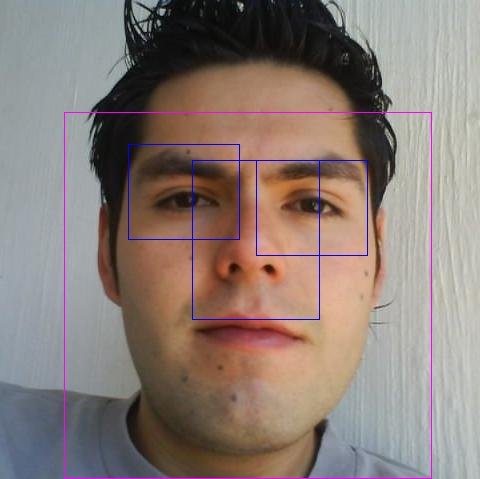
\includegraphics[width=\textwidth]{figures/spec/detected_cff0618f-f631-4b0d-80d9-f582fee46fad}
      \caption{Score=1.4313}
      \label{fig:spec:fd:good_detected1}
    \end{subfigure}
    \begin{subfigure}[b]{0.3\textwidth}
      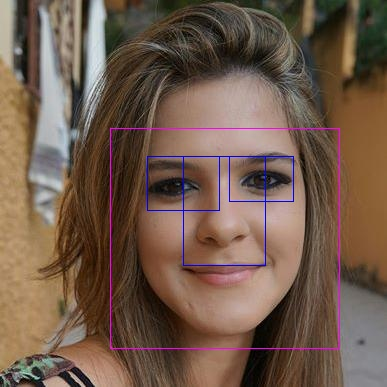
\includegraphics[width=\textwidth]{figures/spec/detected_50508cb1-814e-4374-bf07-cef5c301c3c0}
      \caption{Score=1.20387}
      \label{fig:spec:fd:good_detected2}
    \end{subfigure}
    \begin{subfigure}[b]{0.3\textwidth}
      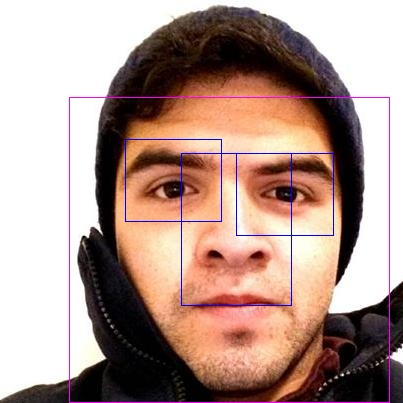
\includegraphics[width=\textwidth]{figures/spec/detected_da153846-1afe-4b36-880a-bf8764bfd935}
      \caption{Score=1.09232}
      \label{fig:spec:fd:good_detected3}
    \end{subfigure}
\caption{Three examples of high-scoring face detections.}
\label{fig:spec:fd:good_detected}
\end{figure}

\begin{figure}
    \centering
    \begin{subfigure}[t]{0.3\textwidth}
      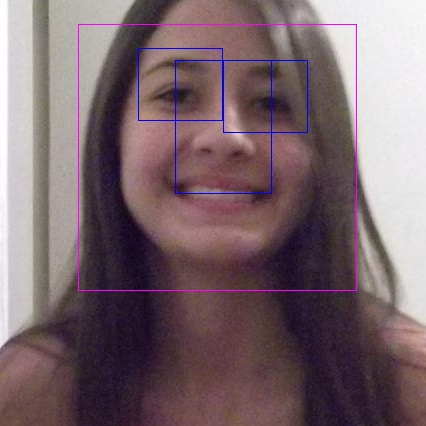
\includegraphics[width=\textwidth]{figures/spec/detected_q3_15c3f02d-31c6-4955-8d05-c05029cdb473}
      \caption{Face detection with score=0.0651244 in upper quartile}
      \label{fig:spec:fd:q3_detected2}
    \end{subfigure}
    \begin{subfigure}[t]{0.3\textwidth}
      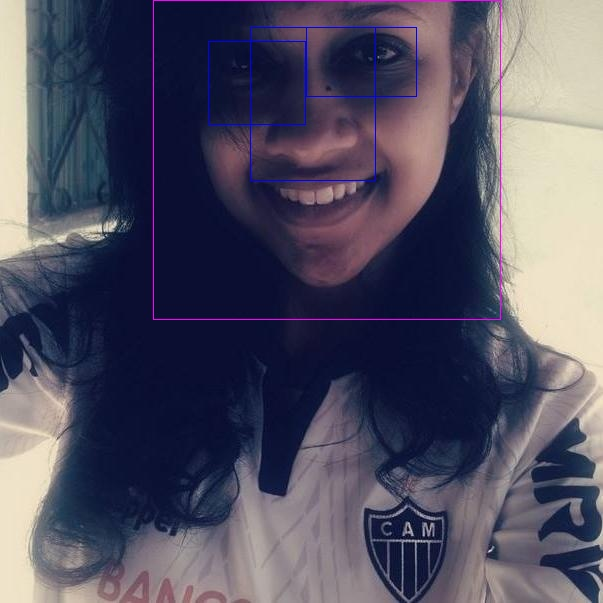
\includegraphics[width=\textwidth]{figures/spec/detected_median_fcb1d3ed-7867-40ba-9691-8cd1f59dc36b}
      \caption{Face detection with score=-0.108765 around the median}
      \label{fig:spec:fd:median_detected1}
    \end{subfigure}
    \begin{subfigure}[t]{0.3\textwidth}
      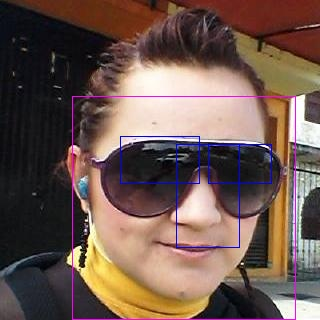
\includegraphics[width=\textwidth]{figures/spec/detected_q1_f1c5f486-1697-4089-9bb6-7962d7db630c}
      \caption{Face detection with score=-0.517613 in lower quartile}
      \label{fig:spec:fd:q1_detected3}
    \end{subfigure}
\caption{Examples of inferior face pictures. Cropped foreheads, blurriness, sunglasses and small faces are some obvious reasons why a face detection might have received a low score.}
\label{fig:spec:fd:other_detected}
\end{figure}

%%% Local Variables: 
%%% mode: latex
%%% TeX-master: "thesis"
%%% End: 


\backmatter

\chapterstyle{default}

\bibliographystyle{plainnat}
\bibliography{bib/all}

\printindex

\chapter{List of Acronyms}
\begin{acronym}\addtolength{\itemsep}{-\baselineskip}
  \acro{PA}{Placeholder Acronym}
\end{acronym}

%%% Local Variables: 
%%% mode: latex
%%% TeX-master: "thesis"
%%% End: 


%\cleartoverso

%\listoffigures

%\cleartoverso

%\listoftables

%\cleartoverso

\end{document}

%%% Local Variables: 
%%% mode: latex
%%% TeX-master: t
%%% End: 
